\chapter{Vyhodnocení tří detektorů stop v pevné fázi}
%ty detektory pocházejí z 8 sady (1., 2. a 3. PDP)

%mikroskop je krytý skleněnou skříňkou
\begin{wrapfigure}{r}{0.42\textwidth}
%\begin{figure}[h]
  \centering
  %\vspace{-20pt}
  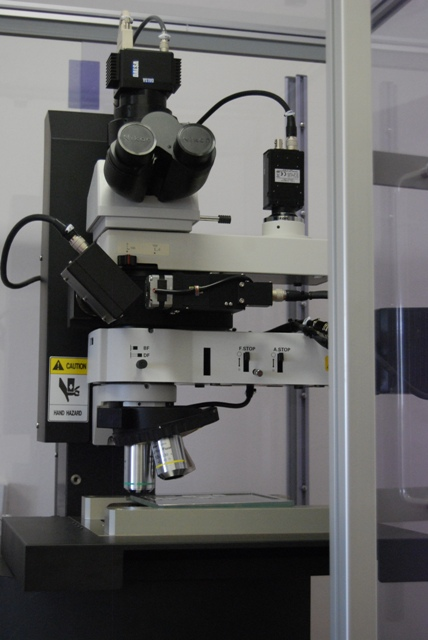
\includegraphics[width=0.4\textwidth]{praktickaCast_mikroskop}
  %\vspace{-20pt}
  \caption{<++> \cite{dosis_HSP1000}}
  \label{fig:praktickaCast_mikroskop}
  %\vspace{-10pt}
%\end{figure}
\end{wrapfigure}

\begin{figure}[h]
  \centering
  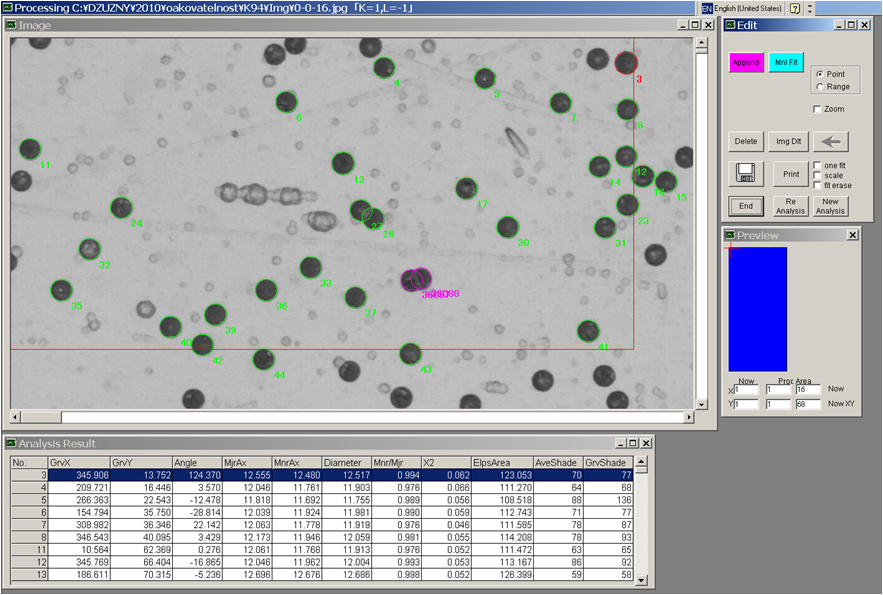
\includegraphics[width=0.85\textwidth]{praktickaCast_hspfit}
  \caption{<++> \cite{dosis_HSP1000}}
  \label{fig:praktickaCast_hspfit}
\end{figure}

\begin{figure}[h]
  \centering
  \begin{subfigure}{0.7\textwidth}
	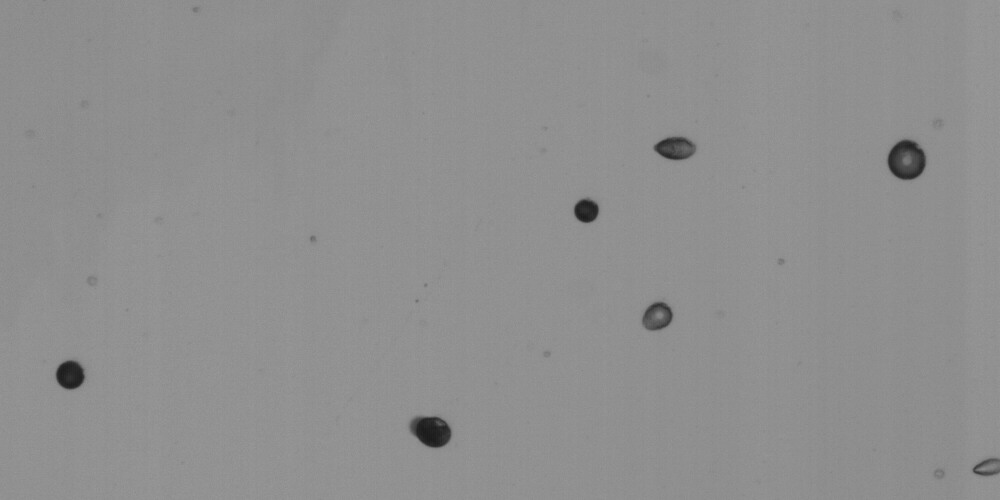
\includegraphics[width=\textwidth]{praktickaCast_stopyOK.jpg}
	\caption{}
  \end{subfigure}
  \begin{subfigure}{0.7\textwidth}
	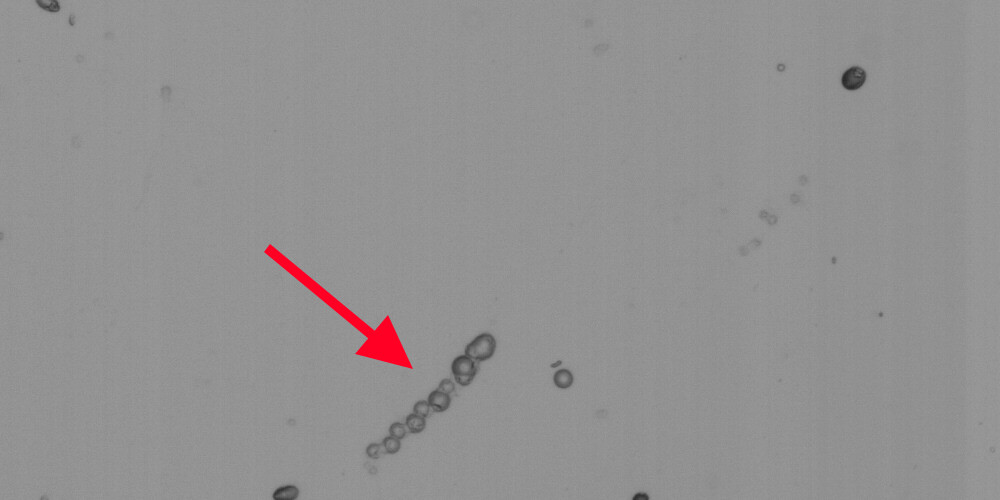
\includegraphics[width=\textwidth]{praktickaCast_stopyNeniStopa1.jpg}
	\caption{}
  \end{subfigure}
  \begin{subfigure}{0.7\textwidth}
	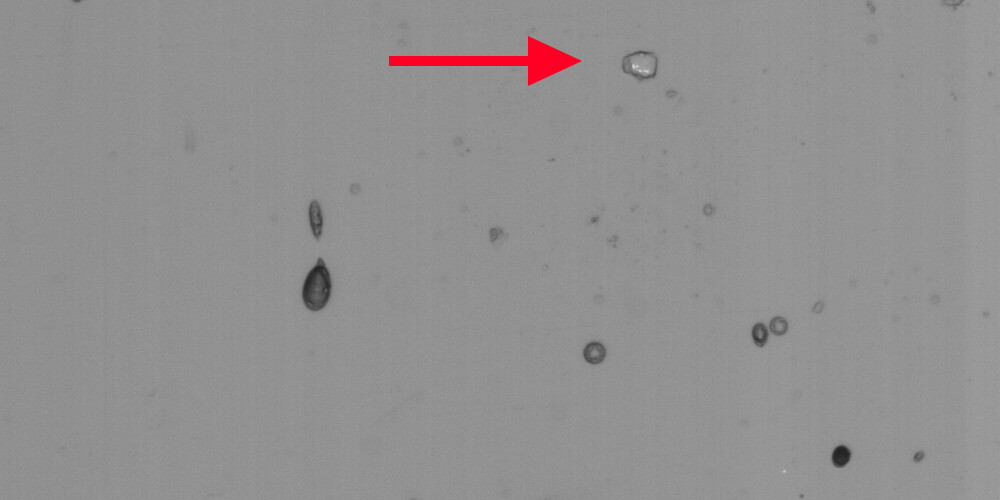
\includegraphics[width=\textwidth]{praktickaCast_stopyNeniStopa2.jpg}
	\caption{}
  \end{subfigure}
  \caption{<+caption text+>}
  \label{fig:praktickaCast_stopy}
\end{figure}

\begin{figure}[h]
  \centering
  \begin{subfigure}{0.7\textwidth}
	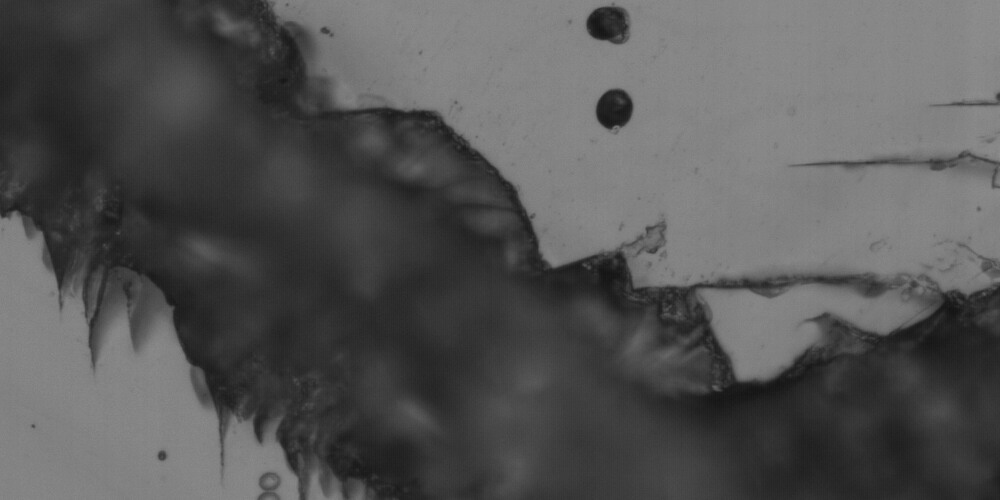
\includegraphics[width=\textwidth]{praktickaCast_stopyPoskozeni1.jpg}
	\caption{}
  \end{subfigure}
  \begin{subfigure}{0.7\textwidth}
	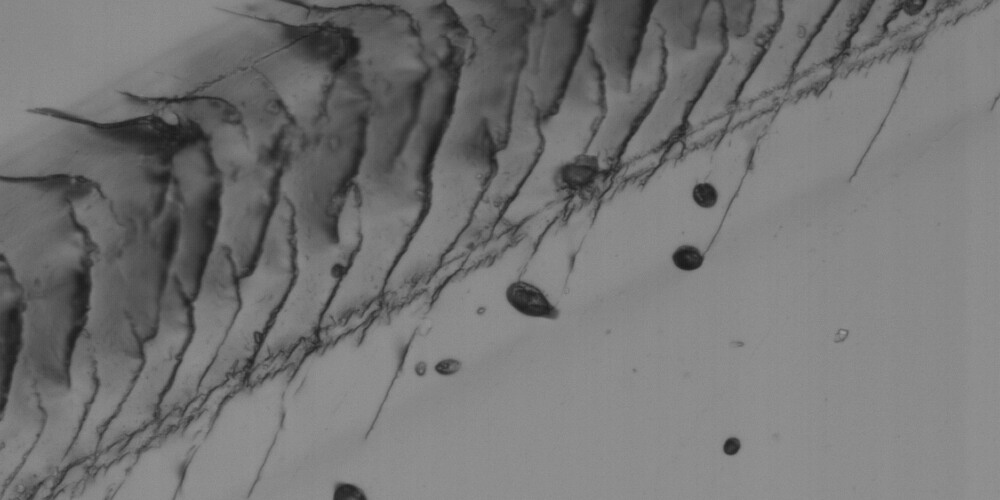
\includegraphics[width=\textwidth]{praktickaCast_stopyPoskozeni2.jpg}
	\caption{}
  \end{subfigure}
  \caption{<+caption text+>}
  \label{fig:praktickaCast_stopyPoskozeni}
\end{figure}

\begin{figure}[h]
  \centering
  \begin{subfigure}{0.49\textwidth}
	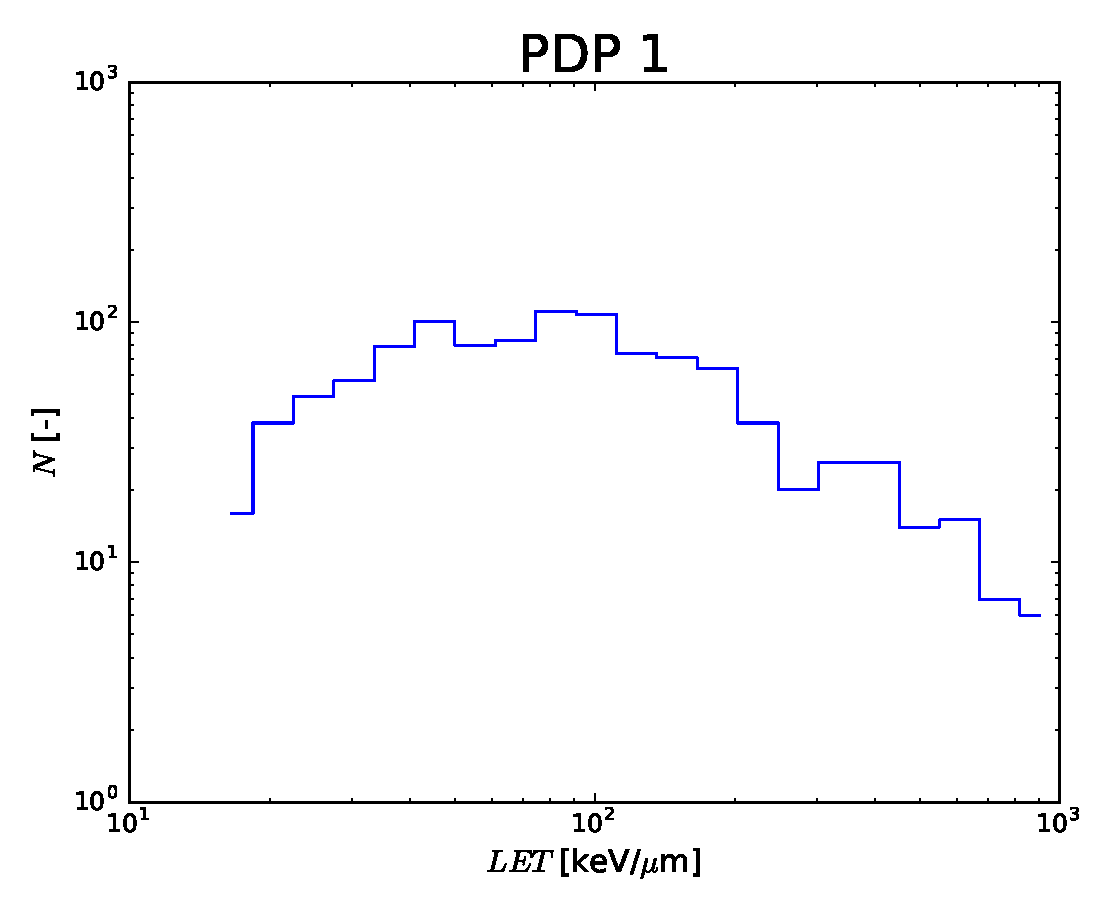
\includegraphics[width=\textwidth]{praktickaCast_spektrum1.eps}
	\caption{}
  \end{subfigure}
  \begin{subfigure}{0.49\textwidth}
	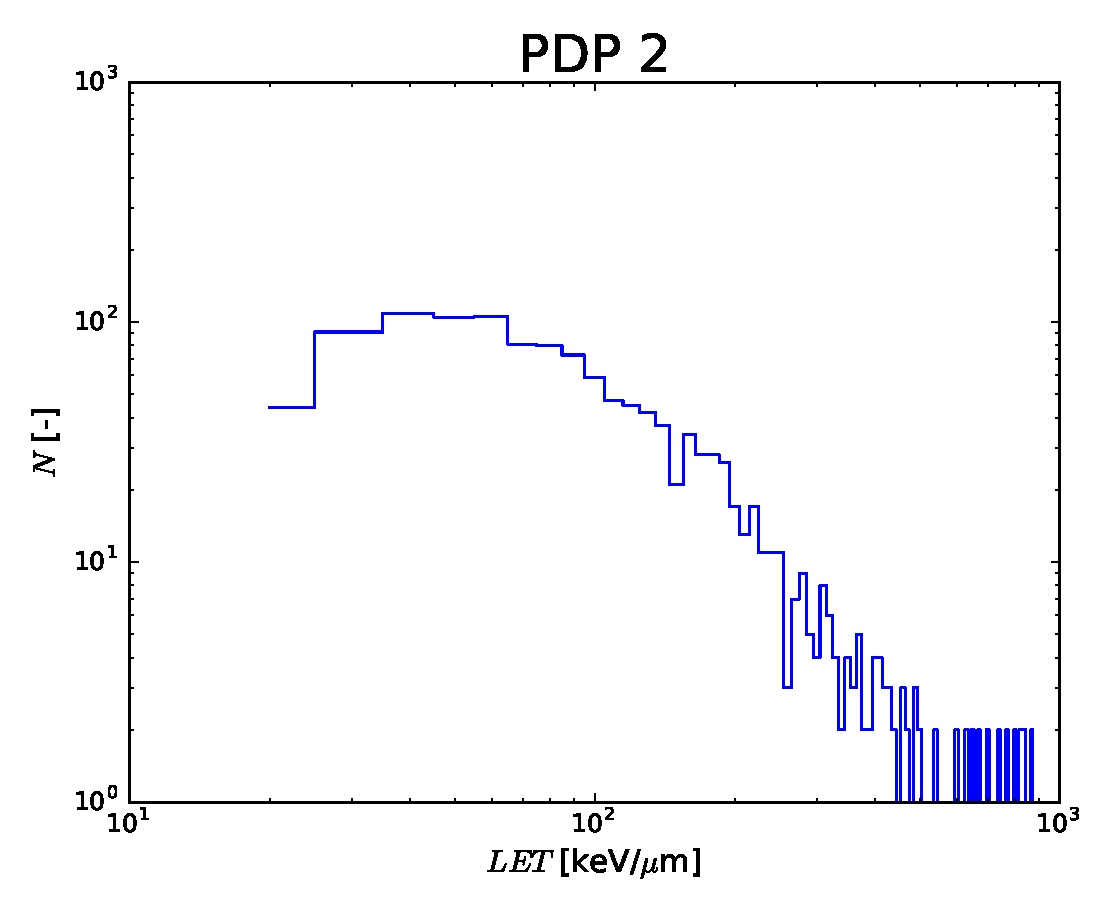
\includegraphics[width=\textwidth]{praktickaCast_spektrum2.eps}
	\caption{}
  \end{subfigure}
  \begin{subfigure}{0.49\textwidth}
	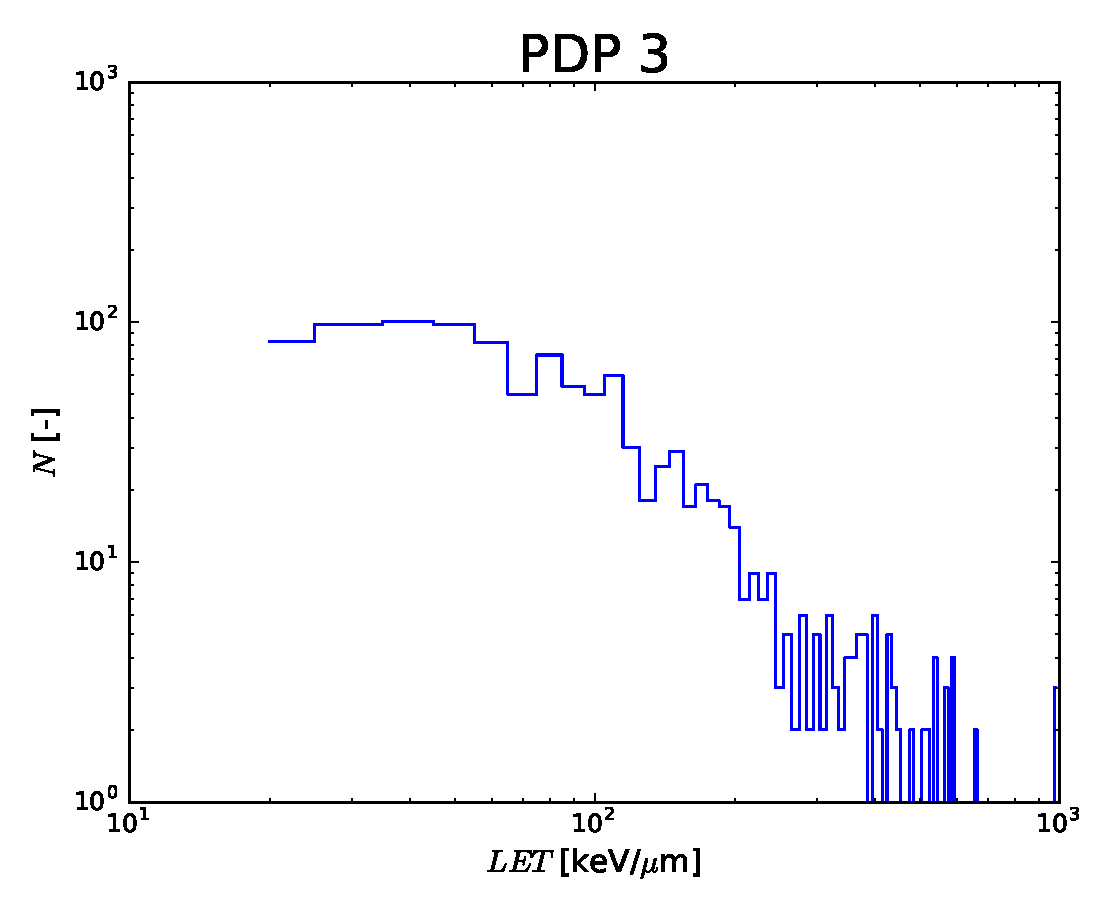
\includegraphics[width=\textwidth]{praktickaCast_spektrum3.eps}
	\caption{}
  \end{subfigure}
  \caption{<+caption text+>}
  \label{fig:praktickaCast_LETspektra}
\end{figure}

%osmá sada
\begin{table}[H]
  \centering
  \begin{tabular}{lll}
	\toprule
	PDP&$D$ [<++>]&$H$ [<++>]\\
	\midrule
	1&5,31501450067&5,31501450067\\
	2&5,068573344&92,5692674847\\
	3&4,31129592097&75,4191405129\\
	\bottomrule
  \end{tabular}
  \caption{<+Caption text+>}
  \label{tab:praktickaCast_davkyVysledky}
\end{table}
